\chapter*{Sperimentazione}
\stepcounter{chapter}
\addcontentsline{toc}{chapter}{Sperimentazione}
\graphicspath{{Chapter6/Chapter6Figs/PNG/}{Chapter6/Chapter6Figs/PDF/}{Chapter6/Chapter6Figs/}}

Una volta in possesso di un framework generale che permetta l'implementazione di strategie arbitrarie, è auspicabile poter disporre di un metodo di valutazione della bontà di tali strategie.\\
Le difficoltà riscontrate nell'affrontare il problema della decisione della mossa da effettuarsi in maniera puramente algoritmica si ripropongono nel momento in cui si voglia applicare lo stesso approccio algoritmico ad un tentativo di valutazione della bontà delle singole mosse.\\
Per questa ragione si è pensato di provare a valutare un giocatore empiricamente in base ai successi conseguiti --- espressi in termini di percentuali di vittorie sul totale delle partite ---  confrontandoli con quelli di un giocatore che abbia una strategia puramente casuale.\\
Si noterà che il numero delle prove eseguite per certe configurazione è piuttosto ridotto; questo è dovuto al fatto che, data la struttura dell'agente giocatore e la fissità della strategia con cui gestisce la fase di asta (fase decisiva nella formazione delle squadre), non è possibile associare a priori la natura (casuale o strategica) di un giocatore al suo ruolo. È stato quindi necessario in alcuni casi condurre un gran numero di prove per ottenerne una quantità accettabile che rispondesse all'interesse sperimentale.


\section{Random vs Random}

Per ottenere un indice di confronto da cui partire si sono innanzitutto condotte 30 partite con cinque giocatori a strategia completamente casuale; i risultati ottenuti sono espressi nella figura \ref{pietab:esperimento-random-random}.\\
Si nota immediatamente come in queste condizioni la squadra del chiamante sia decisamente avvantaggiata; volendo provare a dare un'interpretazione a tale fatto si può avanzare l'ipotesi per cui, mentre la squadra del chiamante sfrutta appieno il vantaggio derivato dalla fase dell'asta (che viene sempre e comunque effettuata in maniera oculata anche nel caso dei giocatori random), costituito dall'avere in mano le carte migliori, la squadra dei villani non ricorre al vantaggio derivato dalla propria superiorità numerica che potrebbe essere invece sfruttato facendo gioco di squadra.\\
Va inoltre considerato che anche nella tradizione è convinzione comune che una buona conduzione della fase dell'asta porti alla squadra del chiamante un considerevole vantaggio rispetto alla squadra avversaria.

% \begin {table}
% \begin{center}
%   \begin{tabular*}{1\textwidth}{@{\extracolsep{\fill}} | c | c | c | }
%     \hline
%                     chiamante + socio & villani & pareggi   \\ \hline
%                     66.7 \% & 30 \% & 3.3 \%              \\ \hline 
%   \end{tabular*}
%   \caption {Percentuali di vittorie in base alla squadra} \label{tab:esperimento-random-random} 
% \end{center}
% \end {table}
%
\def\angle{0}
\def\radius{3}
\def\cyclelist{{"blue","red","green","orange","white"}}
\newcount\cyclecount \cyclecount=-1
\newcount\ind \ind=-1
\begin{figure}[t]
\centering

\subfigure[Percentuale di vittorie conseguite per squadra]{
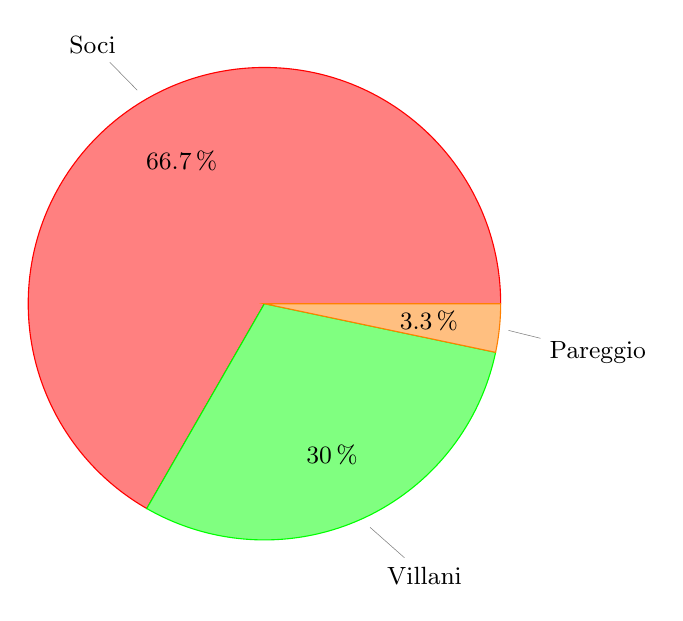
\begin{tikzpicture}[scale=1]
   \small
  \foreach \percent/\name in {
      66.7/Soci,
      30/Villani,
      3.3/Pareggio
    } {
      \ifx\percent\empty\else               % If \percent is empty, do nothing
        \global\advance\cyclecount by 1     % Advance cyclecount
        \global\advance\ind by 1            % Advance list index
        \ifnum3<\cyclecount                 % If cyclecount is larger than list
          \global\cyclecount=0              %   reset cyclecount and
          \global\ind=0                     %   reset list index
        \fi
        \pgfmathparse{\cyclelist[\the\ind]} % Get color from cycle list
        \edef\color{\pgfmathresult}         %   and store as \color
        % Draw angle and set labels
        \draw[fill={\color!50},draw={\color}] (0,0) -- (\angle:\radius)
          arc (\angle:\angle+\percent*3.6:\radius) -- cycle;
        \node at (\angle+0.5*\percent*3.6:0.7*\radius) {\percent\,\%};
        \node[pin=\angle+0.5*\percent*3.6:\name]
          at (\angle+0.5*\percent*3.6:\radius) {};
        \pgfmathparse{\angle+\percent*3.6}  % Advance angle
        \xdef\angle{\pgfmathresult}         %   and store in \angle
      \fi
    };
\end{tikzpicture}
\label{pie:esperimento-random-random}
}

\subfigure[Numero assoluto di vittorie conseguite per squadra su un totale di 30 partite]{
 \begin{tabular*}{1\textwidth}{@{\extracolsep{\fill}} | c | c | c | c | }
    \hline
                    chiamante + socio & villani & pareggi & totale prove svolte   \\ \hline
                    20  & 9  & 1 & 30               \\ \hline 
  \end{tabular*}
  \label{tab:esperimento-random-random}

}

\caption {Random vs Random: esiti delle partite in base alla squadra di appartenenza} \label{pietab:esperimento-random-random} 
\end{figure}




\section{Un giocatore a strategia vs Random}

Nel secondo esperimento condotto si sono giocate 50 partite nelle quali un solo giocatore utilizzava il sistema a strategia mentre tutti gli avversari giocavano casualmente.\\
I risultati sono espressi nella figura \ref{pietab:esperimento-strat-random}.\\
Mentre l'incremento di vittorie da parte della squadra del chiamante era abbastanza atteso, stupisce a prima vista il netto peggioramento della squadra dei compari, che risulta avere più successo se composta da giocatori del tutto casuali rispetto ad averne uno che segua delle strategie.\\
Questo fatto è però facilmente spiegabile tramite l'osservazione per cui le strategie implementate assumono la complicità dei propri compagni di squadra; per esempio, un villano che si trovi a giocare per terzo, prima dei suoi compagni, molto probabilmente giocherà il carico di maggior valore che possiede in mano, sicuro che uno dei propri compagni abbia la possibilità di prenderlo.
Se però questi compagni giocano casualmente è facile che lascino i punti alla squadra avversaria.


\begin{figure}[t]
\centering
\subfigure[Suddivisione delle partite in base alla squadra di appartenenza del giocatore a strategie]{
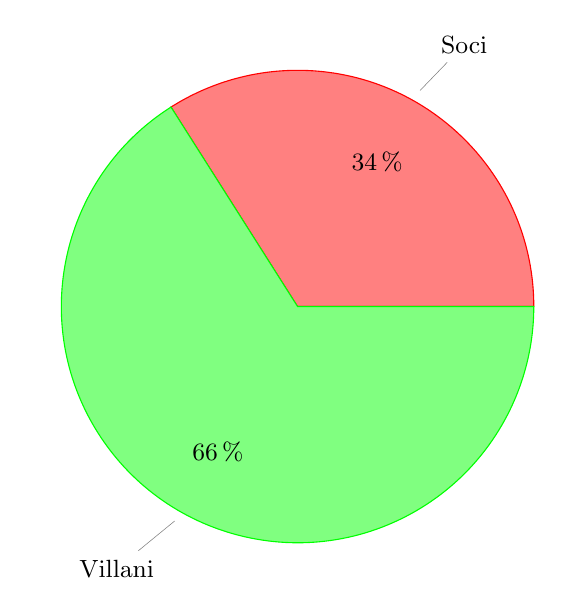
\begin{tikzpicture}[scale=1]
   \small
  \foreach \percent/\name in {
      34/Soci,
      66/Villani
    } {
      \ifx\percent\empty\else               % If \percent is empty, do nothing
        \global\advance\cyclecount by 1     % Advance cyclecount
        \global\advance\ind by 1            % Advance list index
        \ifnum3<\cyclecount                 % If cyclecount is larger than list
          \global\cyclecount=0              %   reset cyclecount and
          \global\ind=0                     %   reset list index
        \fi
        \pgfmathparse{\cyclelist[\the\ind]} % Get color from cycle list
        \edef\color{\pgfmathresult}         %   and store as \color
        % Draw angle and set labels
        \draw[fill={\color!50},draw={\color}] (0,0) -- (\angle:\radius)
          arc (\angle:\angle+\percent*3.6:\radius) -- cycle;
        \node at (\angle+0.5*\percent*3.6:0.7*\radius) {\percent\,\%};
        \node[pin=\angle+0.5*\percent*3.6:\name]
          at (\angle+0.5*\percent*3.6:\radius) {};
        \pgfmathparse{\angle+\percent*3.6}  % Advance angle
        \xdef\angle{\pgfmathresult}         %   and store in \angle
      \fi
    };
\end{tikzpicture}
\label{pie:esperimento-strat-random-1}
}


\subfigure[Esiti delle prove in cui il giocatore a strategie era fra i soci]{%
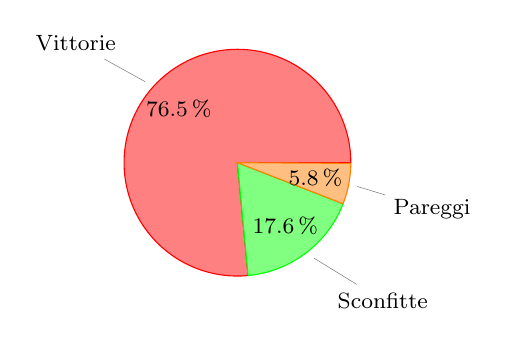
\begin{tikzpicture}[scale=.48]%
\footnotesize%
  \foreach \percent/\name in {%
      76.5/Vittorie,%
      17.6/Sconfitte,%
      5.8/Pareggi%
    }{%
      \ifx\percent\empty\else%               % If \percent is empty, do nothing
        \global\advance\cyclecount by 1%     % Advance cyclecount
        \global\advance\ind by 1%            % Advance list index
        \ifnum3<\cyclecount%                 % If cyclecount is larger than list
          \global\cyclecount=0%              %   reset cyclecount and
          \global\ind=0%                     %   reset list index
        \fi%
        \pgfmathparse{\cyclelist[\the\ind]}% Get color from cycle list
        \edef\color{\pgfmathresult}%         %   and store as \color
        % Draw angle and set labels
        \draw[fill={\color!50},draw={\color}] (0,0) -- (\angle:\radius)%
          arc (\angle:\angle+\percent*3.6:\radius) -- cycle;%
        \node at (\angle+0.5*\percent*3.6:0.7*\radius) {\percent\,\%};%
        \node[pin=\angle+0.5*\percent*3.6:\name]%
          at (\angle+0.5*\percent*3.6:\radius) {};%
        \pgfmathparse{\angle+\percent*3.6}%  % Advance angle
        \xdef\angle{\pgfmathresult}%         %   and store in \angle
      \fi%
    };%
\end{tikzpicture}%
   \label{pie:esperimento-strat-random-1-soci}%
}%
\hfill
\subfigure[Esiti delle prove in cui il giocatore a strategie era fra i villani]{%
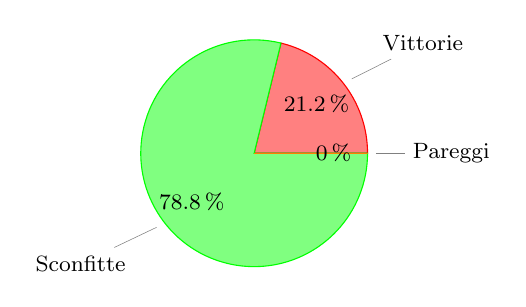
\begin{tikzpicture}[scale=.48]%
\footnotesize%
  \foreach \percent/\name in {%
      21.2/Vittorie,%
      78.8/Sconfitte,%
      0/Pareggi%
    } {%
      \ifx\percent\empty\else%               % If \percent is empty, do nothing
        \global\advance\cyclecount by 1%     % Advance cyclecount
        \global\advance\ind by 1%            % Advance list index
        \ifnum3<\cyclecount%                 % If cyclecount is larger than list
          \global\cyclecount=0%              %   reset cyclecount and
          \global\ind=0%                     %   reset list index
        \fi%
        \pgfmathparse{\cyclelist[\the\ind]}% Get color from cycle list
        \edef\color{\pgfmathresult}%         %   and store as \color
        % Draw angle and set labels
        \draw[fill={\color!50},draw={\color}] (0,0) -- (\angle:\radius)%
          arc (\angle:\angle+\percent*3.6:\radius) -- cycle;%
        \node at (\angle+0.5*\percent*3.6:0.7*\radius) {\percent\,\%};%
        \node[pin=\angle+0.5*\percent*3.6:\name]%
          at (\angle+0.5*\percent*3.6:\radius) {};%
        \pgfmathparse{\angle+\percent*3.6}%  % Advance angle
        \xdef\angle{\pgfmathresult}%         %   and store in \angle
      \fi%
    };%
\end{tikzpicture}%
   \label{pie:esperimento-strat-random-1-vill}%
}%




\subfigure[Esiti delle partite in valore assoluto]{
 \begin{tabular*}{.8\textwidth}{@{\extracolsep{\fill}} | c | c | c | }
    \hline
                  & soci   & villani   \\ \hline
         vittorie & 13     & 7         \\ \hline
         sconfitte& 3      & 26        \\ \hline
         pareggi  & 1      & 0         \\ \hline
         totale   & 17     & 33        \\ \hline 
         
  \end{tabular*}
  \label{tab:esperimento-strat-random}

}




\caption {Un giocatore a strategia vs Random: esiti delle partite in base alla squadra di appartenenza} \label{pietab:esperimento-strat-random} 
\end{figure}




% \begin {table}
% \begin{center}
% \centering
%   \begin{tabular*}{1\textwidth}{@{\extracolsep{\fill}} | p{0.45\linewidth} | p{0.45\linewidth} | @{} }
%     \hline
%                     chiamante + socio & villani    \\ \hline
%                     76.5 \% & 21.2 \%               \\ \hline 
%   \end{tabular*}
%   \caption {Percentuale di vittorie conseguite da ogni squadra con un solo giocatore a strategie} \label{tab:esperimento-uno} 
% \end{center}
% \end {table}


\section{Una squadra a strategia vs Random}

Infine si sono condotte 170 partite con due giocatori a strategia, ottenendone 10 in cui entrambi i giocatori fossero nella squadra dei soci e 115 con tre giocatori a strategia ottenendone 10 in cui fossero tutti tra i villani.
In questo modo è stato possibile valutare le prestazioni di una squadra (sia essa dei villani o dei soci) a strategie contro una random.


Confrontando i risultati di questo esperimento, illustrati nella tabella \ref{tab:esperimento-ultimo}, con quelli ottenuti con squadre a giocatori casuali, (\ref{pie:esperimento-random-random}), è immediato notare come, per entrambe le squadre, ci sia stato un notevole vantaggio derivato dall'adozione (da parte dell'intera squadra) delle strategie basi finora implementate.
\\Questo ha infatti portato a un incremento del 13.3 \% di vittorie sul numero assoluto di partite per la squadra del chiamante e del 30 \% per la squadra dei villani, che equivale addirittura al doppio della percentuale di partite vinte dalla stessa squadra formata da giocatori a strategia casuale.
\begin {table}
\begin{center}
\centering
  \begin{tabular*}{1\textwidth}{@{\extracolsep{\fill}} | p{0.45\linewidth} | p{0.45\linewidth} | @{} }
  
    \hline
                    chiamante + socio & villani    \\ \hline
                    80 \% &  60\%               \\ \hline 
  \end{tabular*}
  \caption {Percentuale di vittorie conseguite, per ogni tipo di squadra, da una squadra di giocatori a strategie contro una a giocatori casuali} \label{tab:esperimento-ultimo} 
\end{center}
\end {table}

\section{Interpretazione dei dati sperimentali}

A causa dell'impossibilità di decidere a priori la formazione delle squadre e, quindi, i ruoli ricoperti dai giocatori di una particolare natura --- a strategia o casuali ---, è stato necessario condurre molte più prove di quante fossero effettivamente utili ai nostri scopi, con la conseguenza di un numero limitato di queste ultime. \\
Inoltre è importante ribadire come le regole implementate siano estremamente basilari, arbitrarie e in numero ridotto (una trentina) data la loro funzione esemplificativa piuttosto che competitiva.\\
Nonostante queste considerazioni l'incremento di prestazioni ottenuto dal giocatore a strategia rispetto a quello random è nettamente visibile. \\
Questa osservazione ci fa concludere che il sistema sia potenzialmente valido e che aumentando l'ampiezza dell'insieme delle strategie, anche tramite l'uso dell'interfaccia per l'utente esperto, sia possibile ottenere giocatori sempre più performanti in questo tipo di valutazione.


% \newcommand{\slice}[4]{
%   \pgfmathparse{0.5*#1+0.5*#2}
%   \let\midangle\pgfmathresult
%
%   % slice
%   \draw[thick,fill=black!10] (0,0) -- (#1:1) arc (#1:#2:1) -- cycle;
%
%   % outer label
%   \node[label=\midangle:#4] at (\midangle:1) {};
%
%   % inner label
%   \pgfmathparse{min((#2-#1-10)/110*(-0.3),0)}
%   \let\temp\pgfmathresult
%   \pgfmathparse{max(\temp,-0.5) + 0.8}
%   \let\innerpos\pgfmathresult
%   \node at (\midangle:\innerpos) {#3};
% }





































